\documentclass[letterpaper,11pt]{article}

\usepackage{amsmath}
\usepackage{amssymb}
\usepackage[hmargin=1.25in,vmargin=1in]{geometry}
\usepackage{booktabs}
\usepackage{graphicx}
\usepackage{hyperref}
\usepackage{lmodern}
\usepackage{microtype}
\usepackage{subcaption}

\title{Coursework 3: STAT 570}
\author{Philip Pham}
\date{\today}

\begin{document}
\maketitle

\begin{enumerate}
\item Consider the Poisson-gamma random effects model given by
  \begin{align}
    Y_i \mid \mu_i, \theta_i
    &\sim \operatorname{Poisson}\left(\mu_i\theta_i\right) \\
    \theta_i
    &\sim \operatorname{Gamma}\left(b, b\right),
  \end{align}
  which leads to a negative binomial marginal model with the variance a
  quadratic function of the mean. Design a simulation study, along the lines of
  that which produced Table 2.3 in the book (overdispersed Poisson example) to
  investigate the efficiency and robustness under
  \begin{itemize}
  \item a Poisson model;
  \item quasi-likelihood with $\mathbb{E}\left[Y\right] = \mu$ and
    $\operatorname{Var}\left(Y\right) = \alpha\mu$; and
  \item sandwich estimation.
  \end{itemize}

  Use a log-linear model
  \begin{equation}
    \log \mu_i = \beta_0 + \beta_1x_i,
  \end{equation}
  with $x_i \sim_\mathrm{iid} \mathcal{N}\left(0, 1\right)$ for
  $i = 1,2,\ldots,n$, and $\beta_0 = -2$ and $\beta_1 = \log 2$.

  Simulate for:
  \begin{itemize}    
  \item $b \in \left\{0.2,1,10,1000\right\}$.
  \item $n \in \left\{10, 20, 50, 100, 250\right\}$.
  \end{itemize}

  Summarize what your take away message is after carrying out these simulations.

  \begin{description}
  \item[Solution:] Note that
    \begin{align}
      \mathbb{P}\left(
      Y_i = y \mid \mu_i
      \right)
      &= \int_0^\infty\mathbb{P}\left(
      Y_i = y \mid \mu_i, \theta_i = \theta
      \right)\mathbb{P}\left(
      \theta_i = \theta
      \mid b
        \right)
        \,\mathrm{d}\theta \nonumber\\
      &= \int_0^\infty
        \left(
        \frac{\left(\mu_i\theta\right)^y}{y!}\exp\left(-\mu_i\theta\right)
        \right)
        \left(
        \frac{b^b}{\Gamma(b)}\theta^{b-1}
        \exp\left(-b\theta\right)
        \right)        
        \,\mathrm{d}\theta \nonumber\\
      &= \frac{\mu_i^y b^b}{y!\Gamma(b)}
        \int_0^\infty
        \theta^{b + y - 1}\exp\left(-\theta(b + \mu_i)\right)
        \,\mathrm{d}\theta \nonumber\\
      &= \frac{\Gamma(y + b)}{y!\Gamma(b)}
        \frac{\mu_i^y b^b}{\left(\mu_i + b\right)^{b + y}}
        = \frac{\Gamma(y + b)}{y!\Gamma(b)}
        \left(\frac{b}{\mu_i + b}\right)^b
        \left(\frac{\mu_i}{\mu_i + b}\right)^y
        \nonumber\\
      &\sim \operatorname{NegativeBinomial}\left(
        b,
        \frac{\mu_i}{\mu_i + b}
        \right).
        \label{eqn:p1_negative_binomial}
    \end{align}

    By properties of the negative binomial distribution, we have that
    \begin{align}
      \mathbb{E}\left[
      Y_i
      \mid x_i
      \right]
      &= \mu_i = \exp\left(\beta_0 + \beta_1x_i\right) \nonumber\\
      \operatorname{Var}\left(Y_i \mid x_i\right)
      &= \mu_i\left(
        1 + \frac{\mu_i}{b}
        \right).
      \label{eqn:p1_y_mean_variance}
    \end{align}
    Thus, smaller values of $b$ correspond to more dispersion.

    \subsection*{Poisson Model}

    In the Poisson model, we assume that
    $\operatorname{Var}\left(Y_i \mid x_i\right) = \mu_i$, e.g.
    $b \rightarrow \infty$, so we neglect the overdispersion parameter.

    In this case, the log-likelihood function is
    \begin{equation}
      l\left(\beta\right) =
      \sum_{i=1}^n\left[
        y_i\left(\beta_0 + \beta_1x_i\right) -
        \exp\left(\beta_0 + \beta_1x_i\right) -
        \sum_{k=1}^{y_i}\log k
      \right],
    \end{equation}
    which gives us the score function
    \begin{equation}
      S\left(\beta\right) = \sum_{i=1}^n\begin{pmatrix}
        y_i - \exp\left(\beta_0 + \beta_1x_i\right) \\
        x_iy_i - x_i\exp\left(\beta_0 + \beta_1x_i\right)
      \end{pmatrix}.
      \label{eqn:p1_score_function}
    \end{equation}
    We can estimate $\beta$ by solving for
    $S\left(\hat{\beta}\right) = \mathbf{0}$, numerically.

    We can estimate the variance of the estimates from the Fisher information,
    \begin{align}
      \operatorname{Var}\left(
      \hat{\beta}
      \right)
      &\approx
        I_n\left(\hat{\beta}\right)^{-1} \label{eqn:p1_beta_hat_variance}\\
      &= \left(
        \sum_{i=1}^n\begin{pmatrix}
          \exp\left(\hat{\beta}_0 + \hat{\beta}_1x_i\right) &
          x_i\exp\left(\hat{\beta}_0 + \hat{\beta}_1x_i\right) \\
          x_i\exp\left(\hat{\beta}_0 + \hat{\beta}_1x_i\right) &
          x_i^2\exp\left(\hat{\beta}_0 + \hat{\beta}_1x_i\right)
        \end{pmatrix} \right)^{-1}  \nonumber\\
      &= \frac{1}{
        \left(\sum_{i=1}^n \hat{\mu}_i\right)\left(\sum_{i=1}^n x_i^2\hat{\mu}_i\right)
        - \left(\sum_{i=1}^n x_i\hat{\mu}_i\right)^2}
        \begin{pmatrix}
          \sum_{i=1}^n x_i^2\hat{\mu}_i &
          -\sum_{i=1}^n x_i\hat{\mu}_i \\
          -\sum_{i=1}^n x_i\hat{\mu}_i &
          \sum_{i=1}^n \hat{\mu}_i
        \end{pmatrix}, \nonumber
    \end{align}
    where $\hat{\mu}_i = \exp\left(\hat{\beta}_0 + \hat{\beta}_1x_i\right)$.
    
    \subsection*{Quasi-likelihood}

    In a quasi-likelihood model, we specify the mean and variance as
    \begin{align}
      \mathbb{E}\left[
      Y_i
      \mid x_i
      \right]
      &= \mu_i = \exp\left(\beta_0 + \beta_1x_i\right) \nonumber\\
      \operatorname{Var}\left(Y_i \mid x_i\right)
      &= \alpha \mu_i
      \label{eqn:p1_y_quasi_mean_variance}
    \end{align}
    From Equation \ref{eqn:p1_y_mean_variance}, we see that this is not quite
    correct, still, but it is closer to the real model than the Poisson model.

    Then, by Equation 2.30 of Wakefield's \emph{Bayesian and Frequentist
      Regression Methods} our estimating function is
    \begin{align}
      U\left(\beta\right)
      &= D^\intercal V^{-1}\left(y - \mu\right)/\alpha \nonumber\\
      &= \sum_{i=1}^n\begin{pmatrix}
        \exp\left(\beta_0 + \beta_1x_i\right) \\
        x_i\exp\left(\beta_0 + \beta_1x_i\right)
      \end{pmatrix}
      \frac{y_i - \exp\left(\beta_0 + \beta_1x_i\right)}{\alpha\exp\left(\beta_0 + \beta_1x_i\right)}
      \nonumber\\
      &= \frac{1}{\alpha}\sum_{i=1}^n\begin{pmatrix}
        y_i - \exp\left(\beta_0 + \beta_1x_i\right) \\
        x_iy_i - x_i\exp\left(\beta_0 + \beta_1x_i\right)
      \end{pmatrix} = \frac{1}{\alpha}S\left(\beta\right)
      \label{eqn:p1_quasi_likelihood_score_function}
    \end{align}
    from Equation \ref{eqn:p1_score_function}. Thus, the maximum
    quasi-likelihood estimate will be the same as the maximum likelihood
    estimate from the Poisson model.

    Having solved for $\hat{\beta}$, we have
    \begin{equation}
      \hat{\mu} = \exp\left(\hat{\beta}_0 + \hat{\beta}_1x_i\right).
      \label{eqn:p1_mu_hat}
    \end{equation}

    by Equation 2.31 of Wakefield's \emph{Bayesian and Frequentist Regression
      Methods}, we can then compute
    \begin{equation}
      \hat{\alpha}_n
      = \frac{1}{n-2}\sum_{i=1}^n \frac{\left(y_i - \hat{\mu}_i\right)^2}{\hat{\mu}_i}
      \label{eqn:p1_alpha_hat}
    \end{equation}

    Then, the variance of our estimates is
    \begin{align}
      \operatorname{Var}\left(
      \hat{\beta}
      \right)
      &\approx
      \hat{\alpha}_n\left(\hat{D}^\intercal \hat{V}^{-1} \hat{D}\right)^{-1} \nonumber\\
      &= \hat{\alpha}_n\left(\sum_{i=1}^n
        \begin{pmatrix}
          \hat{\mu_i} & x_i\hat{\mu_i} \\
          x_i\hat{\mu_i} & x_i^2\hat{\mu_i}.
        \end{pmatrix}\right)^{-1}
        \nonumber\\
      &= \hat{\alpha}_nI_n\left(\hat{\beta}\right)^{-1}
        \label{eqn:p1_beta_hat_quasi_variance}
    \end{align}
    from Equation \ref{eqn:p1_beta_hat_variance}.

    \subsection*{Sandwich Estimation}

    In sandwich estimation, we only need to specify an estimating function
    $G\left(\beta\right)$. Then, we can apply Equation 2.43 of Wakefield's
    \emph{Bayesian and Frequentist Regression Methods} to compute the variance
    of our estimates:
    \begin{align}
      \operatorname{Var}\left(\hat{\beta}\right)
      &= \frac{1}{n}\hat{A}^{-1}\hat{B}\left(\hat{A}^{-1}\right)^\intercal \nonumber\\
      \hat{A}
      &= -\frac{1}{n}\sum_{i=1}^n
        \frac{\partial}{\partial\beta}G\left(\hat{\beta}, X_i, Y_i\right) \nonumber\\
      \hat{B}
      &= \frac{1}{n}\sum_{i=1}^n
        G\left(\hat{\beta}, X_i, Y_i\right)G\left(\hat{\beta}, X_i, Y_i\right)^\intercal.
        \nonumber
    \end{align}

    We can reuse the score function from the quasi-likelihood estimate in
    Equation \ref{eqn:p1_quasi_likelihood_score_function} without $\alpha$, so
    \begin{equation}
      G\left(\hat{\beta}, X_i, Y_i\right)
      = \begin{pmatrix}
        Y_i - \hat{\mu}_i \\
        X_i\left(Y_i - \hat{\mu}_i\right)
      \end{pmatrix}
    \end{equation}
    Thus, our estimate for $\hat{\beta}$ will remain the same.

    From Equations \ref{eqn:p1_beta_hat_variance} and
    \ref{eqn:p1_beta_hat_quasi_variance}, we have that
    \begin{equation}
      \hat{A} = \frac{1}{n}\hat{D}\hat{V}^{-1}\hat{D} = \frac{1}{n}I_n\left(\hat{\beta}\right)
    \end{equation}

    From Equation \ref{eqn:p1_quasi_likelihood_score_function}, we have that
    \begin{align}
      \hat{B}
      &= \frac{1}{n}
        \hat{D}^\intercal\hat{V}^{-1}\operatorname{diag}\left(RR^\intercal\right)\hat{V}^{-1}\hat{D}
      \nonumber\\
      &= \frac{1}{n}\hat{D}^\intercal\begin{pmatrix}
        \frac{\left(y_1 - \hat{\mu}_1\right)^2}{\hat{\mu}_1^2} & & \\
        & \ddots &\\
        & &\frac{\left(y_n - \hat{\mu}_n\right)^2}{\hat{\mu}_n^2}
      \end{pmatrix}\hat{D} =
            \frac{1}{n}\sum_{i=1}^n \frac{\left(y_i - \hat{\mu}_i\right)^2}{\hat{\mu}_i^2}
      \begin{pmatrix}
        \hat{\mu}_i^2 & x_i\hat{\mu}_i^2 \\
        x_i\hat{\mu}_i^2 & x_i^2\hat{\mu}_i^2
      \end{pmatrix} \nonumber\\
      &= \frac{1}{n}\sum_{i=1}^n\left(y_i-\hat{\mu}_i\right)^2
        \begin{pmatrix}
          1 & x_i\\
          x_i & x_i^2
        \end{pmatrix} = \frac{1}{n}\sum_{i=1}^n
                G\left(\hat{\beta},x_i,y_i\right)G\left(\hat{\beta},x_i,y_i\right)^\intercal.
    \end{align}
    
  \end{description}

\item The data in Table \ref{tab:p2_data} contain data on a typical reliability
  experiment and give the failure stresses (in GPa) of four samples of carbon
  fibers of lengths 1, 10, 20 and 50mm.

  \begin{table}
    \tiny
    \centering
    \begin{tabular}{rrrrrrrrrrrrrr}
\toprule
 Length (mm) &      0 &      1 &      2 &      3 &      4 &      5 &      6 &      7 &      8 &      9 &     10 &     11 &     12 \\
\midrule
           1 &  2.247 &  2.640 &  2.842 &  2.908 &  3.099 &  3.126 &  3.245 &  3.328 &  3.355 &  3.383 &  3.572 &  3.581 &  3.681 \\
          10 &  1.901 &  2.132 &  2.203 &  2.228 &  2.257 &  2.350 &  2.361 &  2.396 &  2.397 &  2.445 &  2.454 &  2.454 &  2.474 \\
          20 &  1.312 &  1.314 &  1.479 &  1.552 &  1.700 &  1.803 &  1.861 &  1.865 &  1.944 &  1.958 &  1.966 &  1.997 &  2.006 \\
          50 &  1.339 &  1.434 &  1.549 &  1.574 &  1.589 &  1.613 &  1.746 &  1.753 &  1.764 &  1.807 &  1.812 &  1.840 &  1.852 \\
\bottomrule
\end{tabular}

    \caption{Failure stress data for four groups of fibers.}
    \label{tab:p2_data}
  \end{table}

  \begin{enumerate}
  \item The exponential distribution
    $Y \mid \lambda \sim_\mathrm{iid} \operatorname{Exponential}(\lambda)$, is a
    simple model for reliability data:
    \begin{equation}
      p\left(y \mid \lambda \right) =
      \lambda \exp\left(-\lambda y\right),
      \label{eqn:p2_exponential_pdf}
    \end{equation}
    with $\lambda, y > 0$. The hazard function is the probability of imminent
    failure and is given by
    \begin{equation}
      h\left(y\mid\lambda\right) =
      \frac{p\left(y \mid \lambda\right)}{S\left(y\mid\lambda\right)},
      \label{eqn:p2_hazard_definition}
    \end{equation}
    where
    $S\left(y\mid\lambda\right) = \mathbb{P}\left(Y > y \mid \lambda\right)$ is
    the probability of failure beyond $y$. Derive the hazard function for the
    exponential distribution. Suppose we have a sample $y_1,\ldots,y_n$, of size
    $n$ from an exponential distribution. Find the form of the MLE of $\lambda$
    and the asymptotic variance.
      \begin{description}
      \item[Solution:] The survival function can be derived with Equation
        \ref{eqn:p2_exponential_pdf} as
        \begin{align}
          S\left(y\mid\lambda\right)
          &= \mathbb{P}\left(Y > y \mid \lambda\right) \nonumber\\
          &= \int_y^\infty \lambda \exp\left(-\lambda t\right)\,\mathrm{d}t \nonumber\\
          &= \left. -\exp\left(-\lambda t\right) \right|^\infty_y \nonumber \\
          &= \exp\left(-\lambda y\right).
            \label{eqn:p2_survival}
        \end{align}

        With Equations \ref{eqn:p2_hazard_definition} and \ref{eqn:p2_survival},
        the hazard function is
        \begin{equation}
          h\left(y\mid\lambda\right) =
          \frac{p\left(y \mid \lambda\right)}{S\left(y\mid\lambda\right)}
          = \frac{\lambda \exp\left(-\lambda y\right)}{\exp\left(-\lambda y\right)} = \lambda.
          \label{eqn:p2_hazard}
        \end{equation}
      \end{description}

      Given $y_1,\ldots,y_n$, the log-likelihood function is
      \begin{equation}
        l\left(\lambda\right) = n\log\lambda - \lambda\sum_{i=1}^n y_i.
        \label{eqn:p2_exponential_log_likelihood}
      \end{equation}

      From Equation \ref{eqn:p2_exponential_log_likelihood}, the score function is
      \begin{equation}
        S\left(\lambda\right) = \frac{n}{\lambda} - \sum_{i=1}^n y_i.
        \label{eqn:p2_exponential_score}
      \end{equation}
      Solving $S\left(\hat{\lambda}\right) = 0$, gives use the MLE,
      $\boxed{\hat{\lambda} = \frac{n}{\sum_{i=1}^n y_i} = \frac{1}{\bar{y}}.}$

      The asymptotic variance can be derived from the Fisher information
      \begin{equation}
        I_n\left(\hat{\lambda}\right)
        = \operatorname{Var}\left(S\left(\hat{\lambda}\right)\right)
        = \frac{n}{\hat{\lambda}^2}.
      \end{equation}

      Thus, we have that
      $\boxed{\operatorname{Var}\left(\hat{\lambda}\right) =
        \frac{\hat{\lambda}^2}{n}.}$      
      
    \item For each of the four groups in Table \ref{tab:p2_data}, estimate a
      separate $\lambda$, with an associated standard error. Examine the
      appropriateness of the exponential model via Q-Q plots.

      \begin{description}
      \item[Solution:] The estimates and standard errors for $\lambda$ are in
        Table \ref{tab:p2_exponential_estimates}.

        \begin{table}
          \centering
          \begin{tabular}{rrr}
\toprule
 Length (mm) &  $\hat{\lambda}$ &  Standard error \\
\midrule
           1 &         0.317019 &        0.024386 \\
          10 &         0.432584 &        0.033276 \\
          20 &         0.571253 &        0.043943 \\
          50 &         0.599852 &        0.046142 \\
\bottomrule
\end{tabular}

          \caption{Results of fitting an exponential model for each length.}
          \label{tab:p2_exponential_estimates}
        \end{table}

        From the Q-Q plots in Figure \ref{fig:p2_qq_exponential}, we see that
        the exponential model is a very poor fit for the data. The sampled
        quantiles are very different than the theoretical quantiles. Thus, the
        model appears to be misspecified.

        \begin{figure}
          \centering
          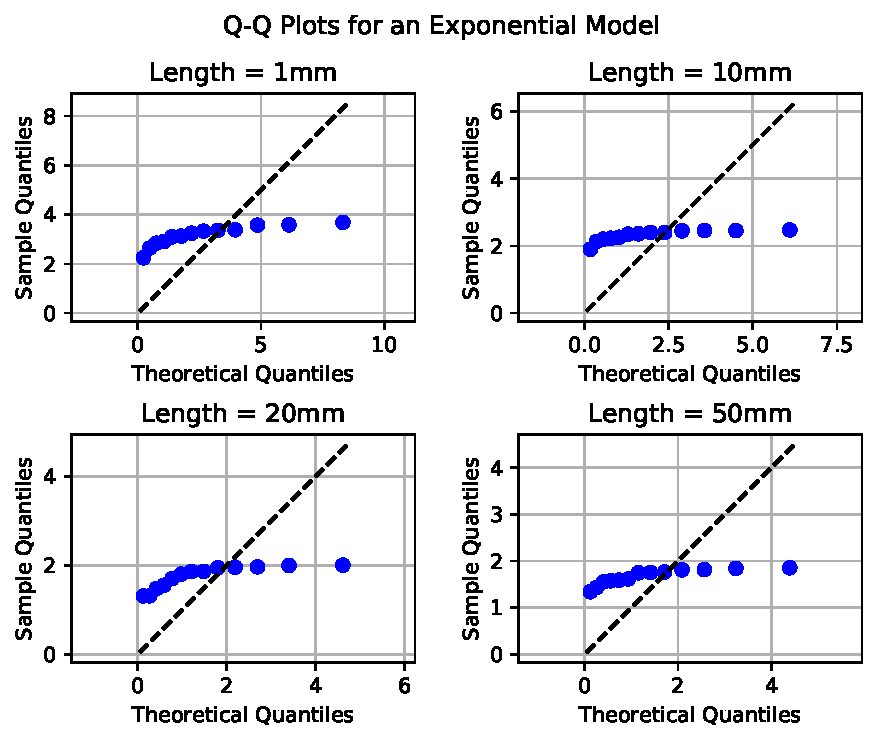
\includegraphics{p2_qq_exponential.pdf}
          \caption{Q-Q plots at each length when fitting an exponential model
            using the MLE.}
          \label{fig:p2_qq_exponential}
        \end{figure}
      \end{description}

      Code for calculations and plots can be found in
      \href{https://nbviewer.jupyter.org/github/ppham27/stat570/blob/master/hw3/failure\_stresses.ipynb}{\texttt{failure\_stresses.ipynb}}.
      
    \item Consider a quasi-likelihood approach to inference for $\lambda$ under
      the model with
      \begin{align}
        \mathbb{E}\left[Y \mid \lambda \right]
        &= \lambda^{-1} \nonumber\\
        \operatorname{Var}\left(Y \mid \lambda\right)
        &= \alpha\lambda^{-2}
        \label{eqn:p2_quasi_likelihood_model}
      \end{align}
      with $\alpha > 0$. Suggest an estimator for $\alpha$.  Estimate $\lambda$,
      $\alpha$, and the standard errors, separately for each of the four groups
      in Table \ref{tab:p2_data}. What do the results suggest to you about the
      fit of the exponential model?

      \begin{description}
      \item[Solution:] The quasi-likelihood score is
        \begin{align}
          U\left(\lambda\right)
          &= D^\intercal V^{-1}
            \left(Y - \mathbb{E}\left[Y \mid \lambda \right]\right)/\alpha \nonumber\\
          &= \begin{pmatrix}
            -\lambda^{-2} & \cdots & -\lambda^{-2}
          \end{pmatrix} \begin{pmatrix}
            \lambda^{2} & & \\
            & \ddots & \\
            & & \lambda^{2}
          \end{pmatrix} \begin{pmatrix}
            \frac{Y_1 - \lambda^{-1}}{\alpha} \\
            \vdots \\
            \frac{Y_n - \lambda^{-1}}{\alpha}
          \end{pmatrix} \nonumber\\
          &= -\frac{1}{\alpha}\sum_{i=1}^n\left(Y_i - \lambda^{-1}\right)
            = -\frac{1}{\alpha}\left(\sum_{i=1}^nY_i - n\lambda^{-1}\right).
            \label{eqn:p2_quasi_score}
        \end{align}
        
        Solving Equation \ref{eqn:p2_quasi_score},
        $U\left(\hat{\lambda}\right) = 0$, we get
        $\hat{\lambda} = \bar{Y}^{-1}$, which is the same as the MLE estimate.

        $\hat{\alpha}$ is given by Equation 2.31 of Wakefield's \emph{Bayesian
          and Frequentist Regression Methods}:
        \begin{equation}
          \hat{\alpha}
          = \frac{1}{n - 1}\sum_{i=1}^n\frac{\left(Y_i - \hat{\mu}\right)^2}{V\left(\hat{\mu}\right)}
          = \frac{\hat{\lambda}^2}{n - 1}\sum_{i=1}^n\left(Y_i - \hat{\lambda}^{-1}\right)^2.
        \end{equation}

        We have that
        \begin{equation}
          \operatorname{Var}\left(U\left(\lambda\right)\right)
          = \mathbb{E}\left[- \frac{\partial U}{\partial \lambda}(\lambda)\right]
          = \frac{n\lambda^{-2}}{\alpha},
        \end{equation}
        we can estimate
        \begin{equation}
          \operatorname{Var}\left(\hat{\lambda}\right) =
          \operatorname{Var}\left(U\left(\hat{\lambda}\right)\right)^{-1}
          \approx \frac{\hat{\alpha}\hat{\lambda}^2}{n},
        \end{equation}
        which is the same as the variance for the MLE estimate multiplied by
        $\hat{\alpha}$. The results of fitting the quasi-likelihood model can be
        seen in Table \ref{tab:p2_quasi_likelihood_estimates}.

        \begin{table}
          \centering
          \begin{tabular}{rrrr}
\toprule
 Length (mm) &  $\hat{\lambda}$ &  $\hat{\alpha}$ &  Standard error ($\hat{\lambda}$) \\
\midrule
           1 &         0.317019 &        0.016873 &                          0.011421 \\
          10 &         0.432584 &        0.005078 &                          0.008550 \\
          20 &         0.571253 &        0.021199 &                          0.023068 \\
          50 &         0.599852 &        0.009633 &                          0.016329 \\
\bottomrule
\end{tabular}

          \caption{Results of fitting a quasi-likelihood model for each length.}
          \label{tab:p2_quasi_likelihood_estimates}
        \end{table}

        From Equation \ref{eqn:p2_quasi_score}, we see that a quadratic variance
        function leads to the same score function as Gamma distribution
        with fixed shape parameter $\alpha^{-1}$ and rate parameter
        $\lambda\alpha^{-1}$. $\alpha = 1$ would correspond to the
        exponential distribution, so it is unsurprising to see that our estimate
        for $\lambda$ is the same as the MLE estimate.

        \begin{figure}
          \centering
          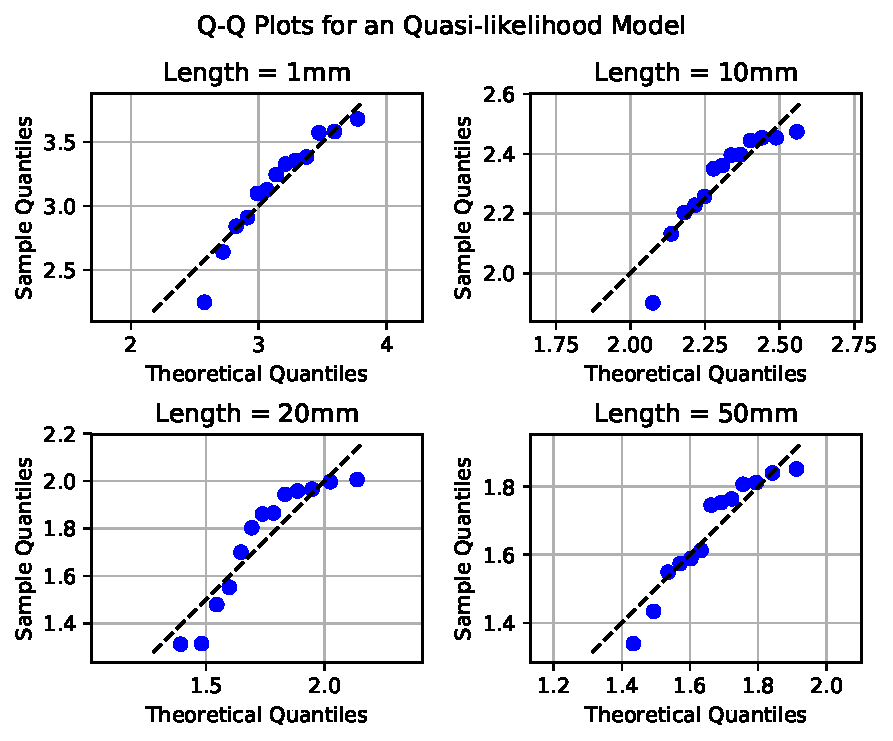
\includegraphics{p2_qq_quasi_likelihood.pdf}
          \caption{Q-Q plots at each length with a Gamma distribution. The shape
            parameter $\hat{\alpha}^{-1}$ and rate parameter
            $\hat{\lambda}\hat{\alpha}^{-1}$ were estimated using
            quasi-likelihood.}
          \label{fig:p2_qq_quasi_likelihood}
        \end{figure}
        
        Standard errors are much smaller than those estimated in Table
        \ref{tab:p2_exponential_estimates}. From Figure
        \ref{fig:p2_qq_exponential}, we see that the residuals are
        underdispersed relative to an exponential model, so $\hat{\alpha} < 1$,
        which leads to the smaller standard error estimates.

        Q-Q plots with the theoretical quantiles derived from
        $\operatorname{Gamma}\left(\hat{\alpha}^{-1},
          \lambda\hat{\alpha}^{-1}\right)$ in Figure
        \ref{fig:p2_qq_quasi_likelihood}. The points lie close the $y = x$
        line. This suggests that the Gamma and quasi-likelihood model are more
        appropriate. They better capture the variance model compared to the
        exponential model.

        Code for calculations and plots can be found in
        \href{https://nbviewer.jupyter.org/github/ppham27/stat570/blob/master/hw3/failure\_stresses.ipynb}{\texttt{failure\_stresses.ipynb}}.
      \end{description}
    \item Obtain the form of the sandwich estimate for the variance of
      $\hat{\lambda}$. Numerically evaluate sandwich standard errors for the
      estimate of $\lambda$ in each of the four groups.

      \begin{description}
      \item[Solution:] We apply Equation 2.43 of Wakefield's \emph{Bayesian and
          Frequentist Regression Methods} to compute the variance of our
        parameter estimate:
    \begin{align}
      \operatorname{Var}\left(\hat{\lambda}\right)
      &= \frac{1}{n}\hat{A}^{-1}\hat{B}\left(\hat{A}^{-1}\right)^\intercal \nonumber\\
      \hat{A}
      &= -\frac{1}{n}\sum_{i=1}^n
        \frac{\partial}{\partial\lambda}G\left(\hat{\lambda}, Y_i\right) \nonumber\\
      \hat{B}
      &= \frac{1}{n}\sum_{i=1}^n
        G\left(\hat{\lambda}, Y_i\right)G\left(\hat{\lambda}, Y_i\right)^\intercal, \nonumber
    \end{align}
    where we resue the quasi-score from Equation \ref{eqn:p2_quasi_score} to
    specify
    \begin{equation}
      G\left(\lambda, Y_i\right) = \frac{1}{\lambda} - Y_i
      \label{eqn:p2_sandwich_score}
    \end{equation}
    as our estimating function.

    Thus, we'll have that
    \begin{align}
      \hat{A}
      &= \frac{1}{n}I\left(\hat{\lambda}\right) = \frac{1}{\hat{\lambda}^2} \nonumber\\
      \hat{B}
      &= \frac{1}{n}\sum_{i=1}^n\left(Y_i - \frac{1}{\hat{\lambda}}\right)^2.
    \end{align}

    Thus, our sandwich estimate will be
    \begin{equation}
      \boxed{
        \operatorname{Var}\left(\hat{\lambda}\right)
        = \frac{\hat{\lambda}^4}{n^2}\sum_{i=1}^n\left(Y_i - \frac{1}{\hat{\lambda}}\right)^2.
      }
      \label{eqn:p2_sandwich_variance}
    \end{equation}
    The results of applying Equations \ref{eqn:p2_sandwich_score} and
    \ref{eqn:p2_sandwich_variance} can be seen in Table \ref{tab:p2_sandwich
      estimates}.   
    
    \begin{table}
      \centering \begin{tabular}{rrr}
\toprule
 Length (mm) &  $\hat{\lambda}$ &  Standard error \\
\midrule
           1 &         0.317019 &        0.010973 \\
          10 &         0.432584 &        0.008215 \\
          20 &         0.571253 &        0.022163 \\
          50 &         0.599852 &        0.015688 \\
\bottomrule
\end{tabular}

      \caption{Results of fitting a model with sandwich estimation for each
        length.}
      \label{tab:p2_sandwich estimates}
    \end{table}

    The estimates for $\hat{\lambda}$ are of course the same as in Tables
    \ref{tab:p2_exponential_estimates} and
    \ref{tab:p2_quasi_likelihood_estimates}, since we reused the same score
    function. The standard errors are smaller than the exponential model since
    the data is underdispersed in that model. However, they are quite similar to
    those in the quasi-likelihood model despite not specifying a variance
    model. From Figure \ref{fig:p2_qq_quasi_likelihood}, we have evidence that
    the quasi-likelihood model fits the data well, so it is unsurprising that an
    empircal estimate would yield similar results.
  \end{description}
\item The Weibull distribution is a common model for survival or reliability
  data:
  $Y \mid \eta,\alpha \sim_\mathrm{iid}
  \operatorname{Weibull}\left(\eta,\alpha\right)$, with $\eta > 0$, and
  $\alpha > 0$. The random variable $Y$ has a Weibull distribution if its
  density can be written in the form
  \begin{equation}
    p\left(y \mid \eta,\alpha\right) = \eta\alpha^{-\eta}y^{\eta-1}\exp\left[
      -\left(\frac{y}{\alpha}\right)^\eta
    \right].
    \label{eqn:p2_weibull_pdf}
  \end{equation}
  
  Find the mean, variance and hazard function of a Weibull distribution. For
  what value of the parameters does the exponential distribution result?

  \begin{description}
  \item[Solution:] The mean can be calculated in terms of the Gamma function
    \begin{align}
      \mathbb{E}\left[
      Y \mid \eta,\alpha
      \right] = \int_0^\infty y p\left(y \mid \eta,\alpha\right)\,\mathrm{d}y
      &= \eta\int_0^\infty \left(\frac{y}{\alpha}\right)^{\eta}
        \exp\left[
        -\left(\frac{y}{\alpha}\right)^\eta
        \right]\,\mathrm{d}y\nonumber\\
      &= \alpha\int_0^\infty u^{1 + 1/\eta - 1}\exp\left(-u\right)\,\mathrm{d}u \nonumber\\
      &= \alpha\Gamma\left(1 + 1/\eta\right).
        \label{eqn:p2_weibull_mean}
    \end{align}

    We can calculate the second moment similarly,
    \begin{align}
      \mathbb{E}\left[
      Y^2 \mid \eta,\alpha
      \right] = \int_0^\infty y^2 p\left(y \mid \eta,\alpha\right)\,\mathrm{d}y
      &= \eta\int_0^\infty y\left(\frac{y}{\alpha}\right)^{\eta}
        \exp\left[
        -\left(\frac{y}{\alpha}\right)^\eta
        \right]\,\mathrm{d}y\nonumber\\
      &= \alpha^2\int_0^\infty u^{2 + 1/\eta - 1}\exp\left(-u\right)\,\mathrm{d}u \nonumber\\
      &= \alpha^2\Gamma\left(2 + 1/\eta\right).
    \end{align}

    Thus, we have that
    \begin{equation}
      \operatorname{Var}\left(
        Y \mid \eta,\alpha
      \right) = \alpha^2\left(
        \Gamma\left(2 + 1/\eta\right) - \left[\Gamma\left(1 + 1/\eta\right)\right]^2
      \right).
    \end{equation}

    The survival function is
    \begin{align}
      S\left(y \mid \eta,\alpha\right)
      &= \int_y^\infty p\left(t \mid \eta,\alpha\right)\,\mathrm{d}t =
        \int_{\left(y/\alpha\right)^\eta}^\infty\exp\left(-u\right)\,\mathrm{d}u \nonumber\\
      &= \exp\left[-\left(\frac{y}{\alpha}\right)^\eta\right].
        \label{eqn:p2_weibull_survival}
    \end{align}

    Thus, the hazard function simplifies to
    \begin{equation}
      h\left(y \mid \eta,\alpha\right) =
      \frac{p\left(y \mid \eta,\alpha\right)}{S\left(y \mid \eta,\alpha\right)} = 
      \eta\alpha^{-\eta}y^{\eta-1}.
      \label{eqn:p2_weibull_hazard}
    \end{equation}

    When $\eta = 1$, this is just the exponential distribution with rate
    parameter $\lambda = \alpha^{-1}$.       
  \end{description}
\item Is the Weibull distribution with unknown parameters $\eta$, $\alpha$ a
  member of the exponential family? What are the implications for inference?
  \begin{description}
  \item[Solution:] No, the Weibull distribution with unknown parameters $\eta$,
    $\alpha$ is not a member of the exponential family. Mainly, if take the
    $\log$ of the probability density function, we have the term
    $\left(\frac{y}{\alpha}\right)^\eta$. This can not be written in the form
    $\theta^\intercal T(y)$, where $\theta$ are parameters and $T(y)$ is a
    transformation of $y$ into a finite-dimensional vector.

    There are implications in inference. The
    \href{https://en.wikipedia.org/wiki/Sufficient_statistic#Exponential\_family}{Pitman-Koopman-Darmois
      theorem} states that only in exponential families is there a sufficient
    statistic whose dimension remains bounded as sample size increases. Thus,
    when inferring the parameters from a sample with maximum likelihood, all the
    data must be used, which may make the computation intractable for large
    datasets. Morever, when doing a Bayesian inference, the posterior must be
    conditioned on all the data rather than a finite set of sufficient
    statistics, so no conjugate prior will exist.

    In particular, generalized linear models require that the response be
    generated from a distribution in the exponential family. The special
    structure of the exponential family make it so the dispersion estimate is an
    ancillary statistic: its estimation is independent of the estimation of the
    mean.
  \end{description}

\item For the Weibull model and a random sample of size $n$ obtain: the
  log-likelihood, the score, and the observed information matrix.

  \begin{description}
  \item[Solution:] The log-likelihood function is
    \begin{equation}
      l\left(\eta,\alpha\right)
      = \sum_{i = 1}^n\left(
        \log\eta - \eta\log\alpha + \left(\eta - 1\right)\log y_i
        - \exp\left[\eta\left(\log y_i - \log\alpha\right)\right]\right)
    \end{equation}

    From which, we have the score function
    \begin{equation*}
      S\left(\eta,\alpha\right) = \sum_{i=1}^n
      \begin{pmatrix}
        \frac{1}{\eta} - \log\alpha + \log y_i -
        \left(\log y_i - \log\alpha\right)
        \exp\left[\eta\left(\log y_i - \log\alpha\right)\right]
        \\
        -\frac{\eta}{\alpha}
        +\frac{\eta}{\alpha}\exp\left[\eta\left(\log y_i - \log\alpha\right)\right]
      \end{pmatrix}.
    \end{equation*}

    The observed information for a single observation is
    \begin{align*}
      I_{y_i}\left(\eta, \alpha\right)
      &= -\nabla \nabla^\intercal l\left(\eta,\alpha\right) = \nabla S\left(\eta,\alpha\right) \\
      &= \begin{pmatrix}
        \frac{1}{\eta^2} + \left(\log \frac{y_i}{\alpha}\right)^2
        \left(\frac{y_i}{\alpha}\right)^\eta
        &
        \frac{1}{\alpha} - \frac{1}{\alpha}\left(\frac{y_i}{\alpha}\right)^\eta -
        \frac{\eta}{\alpha}\left(\log \frac{y_i}{\alpha}\right)\left(\frac{y_i}{\alpha}\right)^\eta
        \\
        \frac{1}{\alpha} - \frac{1}{\alpha}\left(\frac{y_i}{\alpha}\right)^\eta -
        \frac{\eta}{\alpha}\left(\log \frac{y_i}{\alpha}\right)\left(\frac{y_i}{\alpha}\right)^\eta
        &
        -\frac{\eta}{\alpha^2} + \frac{\eta}{\alpha^2}\left(\frac{y_i}{\alpha}\right)^\eta
        + \left(\frac{\eta}{\alpha}\right)^2\left(\frac{y_i}{\alpha}\right)^\eta
      \end{pmatrix}.
    \end{align*}
  \end{description}
\end{enumerate}
\end{enumerate}
\end{document}
